\chapter{Instrukcja wdrożeniowa}
PLiki źródłowe projektu zostały umieszczone w zdalnym repozytorium kodu na stonie github. 
Link do repozytorium: \url{https://github.com/Quarol/Praca-inzynierska.git}

Użytą wersją języka Python jest Python 3.12.4. Aby wykorzystać zaprojektowany system, należy ją zainstalować.

Repozytorium składa się z dwóch plików wykonywalnych (\emph{main.py}, \emph{install\_requirements.py}) oraz dwóch folderów -- \emph{assets} oraz \emph{detector}. Struktura pokazana na ryskunku \ref{fig:repo}.
\begin{figure}
    \centering
    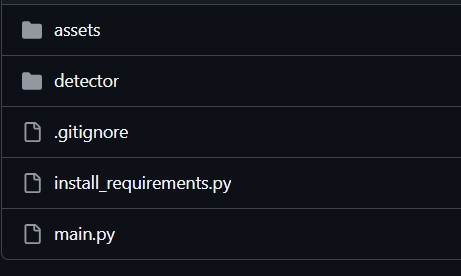
\includegraphics[width=\linewidth]{_repo.jpg}
    \caption{Struktura repozytorium.}
    \label{fig:repo}
\end{figure}

Folder \emph{assets} zawiera plik dźwiękowy służący jako alarm w systemie. Folder \emph{detector} zawiera wsysztkie pliki źródłowe z opisanymi komponentami systemu.

Plik \emph{install\_requirements.py} to skrypt służący do instalacji wszystkich wykorzystanych modułów języka Python w użytych wersjach.

Plik \emph{main.py} jest to plik uruchamiający aplikację.

W celu instalacji modułów, a następnie wystartowania oprogramowania należy wykonań dwie następujące komendy w terminalu:
\begin{lstlisting}
python install_requirements.py
python main.py
\end{lstlisting}


